\chapter{Design of Module \textit{userprog}}


\section{Process Termination Messages \& Argument passing}

    \subsection{Initial Functionality}

	At the beginning of this project the function {\textit{process\_execute()} doesn't support argument passing. We want to implement it so that the main function can be called with arguments.

    \subsection{Data Structures and Functions}

    \begin{lstlisting}

      "In thread.h :"
	
	struct thread {
	    /* The process id to which the thread
	       belongs to. */
	       int pid;
	};

	"In process.h / process.c"

	/* this function return the first substring 
	of the parameter */
	char* firstSubstring( const char* arg, const char delimitator );

	/* this function will add the parameter on the stack.
	First the value are passed in any order. After that will 
	set to the corect aligment, and then pass the address of
	the arguments in reverse order and the number of the arguments.*/
	void passArguments( const char* arg, void* esp );

    \end{lstlisting}


    \subsection{Functionality}

	  Every time when a process is created the method \textit{process\_execute} is called. Will have as parameter the arguments for the new process.The first substring will be the name of the process.We get the first parameter of the argument and set it as the name of the thread that will be created. The initialization of the new thread will be in the other process.

	  The function passArguments has the following pseudocode

    %Here you have a pseudo-code description of an algorithm taken fom \\ \href{http://en.wikibooks.org/wiki/LaTeX/Algorithms\_and\_Pseudocode\#Typesetting\_using\_the\_program\_package}{http://en.wikibooks.org/wiki/LaTeX}. It uses the \textit{program} package. Alternatively, you can use \textit{algorithmic} or \textit{algorithm2e} packages. 

    \begin{program}
    %\mbox{Example of a pseudo-code algorithm description:}
    \BEGIN %
    %  \FOR i:=1 \TO 10 \STEP 1 \DO
    %     |expt|(2,i); \\ |newline|() \OD %
    %\rcomment{This text will be set flush to the right margin}
    %\WHERE
    \PROC |passArguments|(x,s) \BODY
              \DO
		token := strtok\_k( x );
		\IF token= null 
		  \THEN \EXIT 
		  \ELSE push( s, token )   
		\FI;
	      \OD
	      |alligment|(s)
              \FOR i:= 1 \TO numberOfParameters \STEP 1 \DO
		pushAddress( s ) \OD
     \ENDPROC
    \END
    \end{program}


    \subsection{Design Decisions}

	This solution has one advantage. The arguments are deduced by the child process. Because we tokenize the parameter in the method \textit{start\_process} which will be called by the child process. If we had done this in the method \textit{process\_execute} then the tokenizing was made by the parent process and the child process, doesn't process his own resources.

    \subsection{Tests}


      \textbf{args-dbl-space.c}\\
      \textit{Source:} tests/userprog/args-dbl-space.c\\
      \textit{Purpose:} Checks if there are double spaces 
	  in the argument list.


      \textbf{args-many.c}\\
      \textit{Source:} tests/userprog/args-many.c\\
      \textit{Purpose:} Checks if there can be any number of arguments. 
	  The number is greater than 9.

    \textbf{args-multiple.c} \\
    \textit{Source:} tests/userprog/args-multiple.c\\
    \textit{Purpose:} Checks if there are some arguments in 
	  the argument list.

    \textbf{args-none.c}\\
    \textit{Source:} tests/userprog/args-none.c\\
    \textit{Purpose:} Checks if there are 0 arguments.

    \textbf{args-single.c}\\
    \textit{Source:} tests/userprog/args-single.c\\
    \textit{Purpose:} Checks if there is only one argument.\\
    \textit{Description:}
    
\section{System calls}

    \subsection{Initial Functionality}

	At the beginning of this project, pintOS does not provide the posibility of running any kind of user programs, much less make system calls from them. Moreover, there is no data structure to support processes. Our purpose is to implement the data structures required to support processes, as well as making various system calls.

    \subsection{Data Structures and Functions}

    \begin{lstlisting}
    //In process.h :
      
      /* maximum number of processes running at the same 
      time. May need some adjustments. */
      #define MAX_PROCESSES 1024

      /* possible states of a process. 
	  ALIVE  is a process that has still not finished 
		 it's execution. 
	  KILLED is a process killed by the kernel.
	  DEAD 	 is a process that was killed at user's 
		 request by calling exit. */
      enum pstatus_t {ALIVE, KILLED, DEAD}

      struct process_t {
	  /* process id of this process */
	  pid_t pid;				

	  /* pid (process id) of this process's parent */
	  pid_t ppid;				
	  
	  /* status of the process: one of ALIVE, KILLED, 
	     DEAD. */
	  process_status_type status;
      
	  /* the code returned by the process at exit */
	  int exit_code;

	  /* The thread that is waiting after this thread. */
	  struct thread* waiter_thread;

	  /* List of file descriptors. */
	  struct list owned_file_descriptors;
      };
    
      typedef struct process_t processs_t;

      //In process.c: 

      /* The processes table. we need a table with all processes, 
      a hash table will do fine, standard C array too. */
      static process_t processes_table[MAX_PROCESSES];

      //In userprog/syscalls.h: (kernel side)
      
      /* synchronisation lock in order to execute
	 only one syscall at a time */
      static struct lock syscall_lock;

      /* Reads a byte at user virtual address UADDR.
	UADDR must be below PHYS_BASE.
	Returns the byte value if successful, -1 if a 
	segfault occurred. 
	Warning! BYTE is returned as an int.
	Implementation in pintos manual.*/
      static int get_user (const uint8_t *uaddr);

      /* Writes BYTE to user address UDST.
	 UDST must be below PHYS_BASE.
	 Returns true if successful, false if a segfault 
	 occurred. 
	 Implementation in pintos manual.*/
      static bool put_user (uint8_t *udst, uint8_t byte);

    //In exception.c:

    page_fault()

    //In file.h:
    
    /* Structure used to identify an open file through 
       an integer descriptor. */
    struct file_descriptor {

      /* Identifier used in user mode. */
      int id;
      
      /* Reference to the file structure identified 
      through this descriptor. */
      struct file* file_ref;
    
      /* List element used for the process list. */
      struct list_elem elem;
    }
    \end{lstlisting}


    \subsection{Functionality}

    \subsubsection{Filesystem sycall}
    \vspace{-3em} %latex hack
      \begin{program}

	take\_arguments\_from\_stack();
	select\_system\_call();
	
	syscall\_lock.aquire();
	validate\_arguments();
	\IF \text{invalid addresses}
	  \THEN sycall\_lock.release();\text{thread\_exit}
	\FI
	
	\text{copy any user space buffer into a local buffer}
	\text{by checking for each address from the buffer that} 
	\text{it is valid and the buffer does not try to get }
	\text{out of user space }

	\IF \text{invalid addresses}
	  \THEN sycall\_lock.release();\text{thread\_exit}
	\FI

	\text{find file descriptor by id}
	\text{call functions from file.h/filesys.h using local buffers}

	\text{clean memory and release locks}
      \end{program}

    \subsubsection{Validate get from address}
    \vspace{-1em} %latex hack
      \begin{lstlisting}
//similar for put to address : use put_user
//(see section Data structures and functions}

if( address > PHYS_BASE ) //is in kernel space 
  free local buffers & release locks
  thread_exit(); 
else {
  //do not dereference here. just call get_user with address
  int result = get_user( address ) 
  if(result == -1) {
      free local buffers & release locks
      thread_exit(-1)
  }	
  else byte = (uint8_t)result;
}
      \end{lstlisting}

    \subsubsection{Exit sycall}
    \vspace{-3em} %latex hack
      \begin{program}
	syscall\_lock.aquire();
	proc\_crt = get\_process(current\_thread.pid);
	proc\_crt.exit\_code = status;
	thread\_exit() \text{//calls process\_exit};
	proc\_crt.status = DEAD;
      \end{program}
    \begin{lstlisting}
/* Free the current process's resources. */	
   void process_exit (void)
   {
    ..
    process_t crt_process = get_process(current_thread.pid);
    if( crt_process.waiter_thread != NULL ) {
      //after thread_unblock current thread will be destroyed
      //this is why we release the lock before.
      syscall_lock.release();
      thread_unblock( crt_process.waiter_thread );
   }
    \end{lstlisting}


    \subsubsection{wait syscall}
    \vspace{-1em} %latex hack
    \begin{lstlisting}
int
process_wait (pid_t child_pid) 
{
    lock_aquire(&process_wait_lock);
    
    //we test if child_tid is in the table.
    if(child_tid does not exist) 
	return -1;

    if(get_process().id != get_process(child_pid).parent_id)
	return -1;

    int exit_code;

    if(get_process(child_pid).status == KILLED) {
	exit_code = -1;
	
    }
    else if(get_process(child_pid).status == DEAD) {
	exit_code = get_process(child_pid).exit_code;            
    }
    else if(get_process(child_pid).status == RUNNING) {
	thread_block(); 
	exit_code = get_process(child_pid).exit_code;
    }

    clean_process_data(child_pid);
    return exit_code;
}
    \end{lstlisting}


    \subsection{Design Decisions}

	This solution has the advantage that ... 

	On the other hand it is not so good that ... . 

	A better solution would be ... . 

	However, this solution is better than ...

    \subsection{Tests}

    \textbf{wait-twice}\\
      \textit{Source:} tests/userprog/wait-twice\\
      \textit{Purpose:} Checks what happens when we wait twice for the same child process


      \textbf{wait-simple}\\
      \textit{Source:} tests/userprog/wait-simple\\
      \textit{Purpose:} Waits for a child process and checks the exit code

    \textbf{wait-bad-pid} \\
    \textit{Source:} tests/userprog/wait-bad-pid\\
    \textit{Purpose:} Waits for a random pid, that may not be in the process table at all. The wait function should return -1 without waiting.
    
\section{Denying writes to executables}

     \subsection{Initial Functionality}

	At the beginning of this project ... .

    \subsection{Data Structures and Functions}

    \begin{lstlisting}

      "In ... :"
	
	struct structure_def {
	    type field;
	};

	/* comments */
	variable definition;

	/* comments */
	function definition;

    \end{lstlisting}


    \subsection{Functionality}

	

    %\begin{figure}[h]
    %	\centering
    %	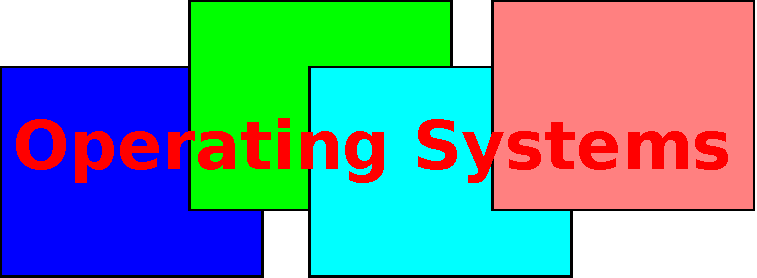
\includegraphics[width=0.5\textwidth]{figures/sample-image.pdf}
    %	\caption{Sample image}
    %	\label{fig:sample-image}
    %\end{figure}


    %Here you have a pseudo-code description of an algorithm taken fom \\ \href{http://en.wikibooks.org/wiki/LaTeX/Algorithms\_and\_Pseudocode\#Typesetting\_using\_the\_program\_package}{http://en.wikibooks.org/wiki/LaTeX}. It uses the \textit{program} package. Alternatively, you can use \textit{algorithmic} or \textit{algorithm2e} packages. 

    %\begin{program}
    %\mbox{Example of a pseudo-code algorithm description:}
    %\BEGIN %
    %  \FOR i:=1 \TO 10 \STEP 1 \DO
    %     |expt|(2,i); \\ |newline|() \OD %
    %\rcomment{This text will be set flush to the right margin}
    %\WHERE
    %\PROC |expt|(x,n) \BODY
    %          z:=1;
    %          \DO \IF n=0 \THEN \EXIT \FI;
    %             \DO \IF |odd|(n) \THEN \EXIT \FI;
    %\COMMENT{This is a comment statement};
    %                n:=n/2; x:=x*x \OD;
    %             \{ n>0 \};
    %             n:=n-1; z:=z*x \OD;
    %          |print|(z) \ENDPROC
    %\END
    %\end{program}


    \subsection{Design Decisions}

	This solution has the advantage that ... 

	On the other hand it is not so good that ... . 

	A better solution would be ... . 

	However, this solution is better than ...

    \subsection{Tests}

    \textbf{name of the test}\\
    \textit{Source:} path/to/test.c\\
    \textit{Purpose:} What does it check?\\
    \textit{Description:} Short description.
    \textit{Solution:(if necessary)} Here, if what the test does is something that was not explicitly asked in the requirements, it would be good to say that we already treat that situation and where. If it's something that should be solved only by the implementation of the requirements you can say: Solved by requirements fulfillment.
